% So we make this "beamer" rather than document!

\documentclass[11pt]{beamer}
% For handout add ,handout after 11pt
% Kill page numbers with [numbering=none] in next line:
\usetheme[sectionpage=none,numbering=none]{metropolis}           % Use metropolis theme
	% To do printouts, add ", handout"  after aspectratio.
\usepackage{makecell}
\usepackage{booktabs}
\usepackage{graphicx}
\usepackage{color}
%\usepackage[utf-8]{inputenc}
\usepackage{bbm}
  \usepackage{bm}
\newcommand{\notimplies}{%
  \mathrel{{\ooalign{\hidewidth$\not\phantom{=}$\hidewidth\cr$\implies$}}}}
\definecolor{violet}{RGB}{223,115,255}
\usepackage{transparent}
\definecolor{cyan2}{RGB}{0,255,255}
\makeatletter
\newcommand\primitiveinput[1]
{\@@input #1 }
\makeatother
\usepackage{tabu}
\usepackage{dcolumn}
\definecolor{Gray}{gray}{0.85}

\usepackage{xcolor,colortbl}


\title{Welcome to MIDS!}
\author{\small Nick Eubank}
\date{\vspace*{.3in} \date}


% This is the beginning of a real document!
\begin{document}


\begin{frame}
\maketitle
\end{frame}


\begin{frame}[c]{What is Data Science?}
\begin{enumerate}
	\pause \item What (\alert{in theory}) do we think Data Science should be?
	\pause \item What (\alert{empirically}) is Data Science?
\end{enumerate}
\end{frame}


\begin{frame}[c]{What (in theory) should Data Science be?}

\pause Study of how to \alert{solve problems} \pause by \alert{answering questions} \pause using \alert{quantitative data.}

\pause
\begin{itemize}
	\item Problem-first approach. 
	\begin{itemize}
		\pause \item Data Science is an \emph{applied} discipline!
	\end{itemize} 
	\pause \item The tool you use should be dictated by the question you seek to answer
\end{itemize}

\end{frame}

\begin{frame}[c]{What (empirically) is Data Science?}

\end{frame}

\begin{frame}[c]{How did Data Science become a thing?}

Over the past several decades:
\begin{enumerate}
	\item Availability of data $\uparrow$
	\item Computational power $\uparrow$
\end{enumerate}
\pause
$\Rightarrow$ Huge proliferation and increase in sophistication of computational methods
\end{frame}


\begin{frame}[c]{How did Data Science become a thing?}

\begin{itemize}
	\item Academic research is organized into silos:
	\pause
	\begin{itemize}
		\item Computer Science
		\item Statistics
		\item Economics
		\item Political science
		\item Engineering
	\end{itemize}
\end{itemize}
\pause $\Rightarrow$ Development of new tools occurred \emph{within} each silo.
\end{frame}


\begin{frame}[c]{Where are we today?}
Very little cross-pollination across silos
\begin{itemize}
	\pause \item Lots of duplication of development.
	\pause \item Every silo has its own vocabulary.
	\pause \item Each silo has focused on the aspects most relevant to their applications. e.g.:
	\begin{itemize}
		\pause \item CS likes to classify things and make predictions, don't care how model works
		\item Social scientists like to make causal statements, don't care about predictive power
	\end{itemize}
\end{itemize}
\end{frame}

\begin{frame}[c]{}
\pause 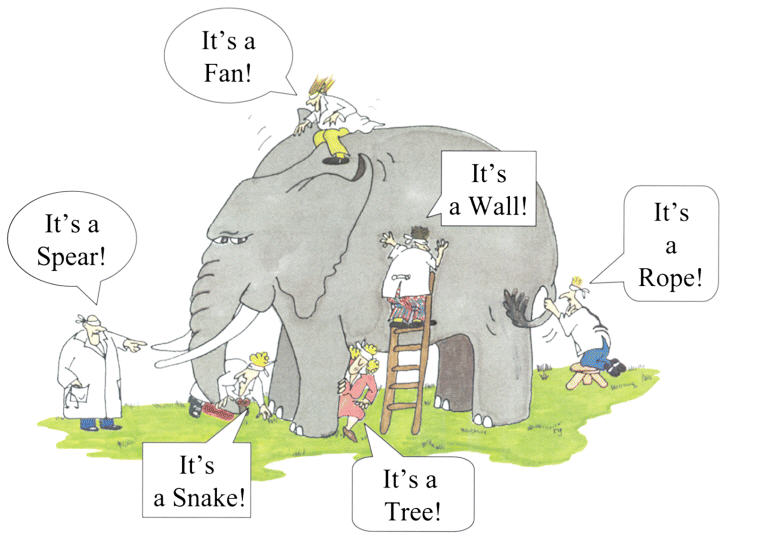
\includegraphics[width=\textwidth]{blindmenelephant.jpg}
\pause $\Rightarrow$ This is where we are \emph{now.}
\end{frame}

\begin{frame}[c]{What is (empirically) Data Science?}
\pause An effort to unify the development of quantitative methods \\
\pause $\rightarrow$ Recognize the elephant
\end{frame}

\begin{frame}[c]{Why does this matter to you?}
\begin{itemize}
	\item Many of you will have a conception of what is (and is not) data science.
	\begin{itemize}
		\pause \item Don't hold to those beliefs too strongly.
	\end{itemize}
	\pause \item MIDS aims to ensure \emph{all} our students have a solid, wide foundational understanding of the discipline.
	\pause \item My people who talk about data science were trained in a single silo, and may not fully recognize what's happening beyond.
	\begin{itemize}
		\pause \item That's why we have faculty from many fields.
	\end{itemize}
\end{itemize}
\end{frame}

\begin{frame}[c]{Areas of Data Science}
	\begin{columns}
	\begin{column}{0.45\textwidth}
		\uncover<1->{\textbf{Software Engineering DS}}
		\begin{itemize}
			\item \uncover<2->{Recommendation engines}
			\item \uncover<2->{Financial trading algorithms}
			\item \uncover<2->{Self-driving cars}
		\end{itemize}
	\end{column}
	\begin{column}{0.5\textwidth}  %%<--- here
		\uncover<1->{\textbf{Data Analysis DS}}
		\begin{itemize}
			\item \uncover<3->{Impact of policy change}
			\item \uncover<3->{Effectiveness of health interventions}
			\item \uncover<3->{Plan political campaigns}
		\end{itemize}
	\end{column}
	\end{columns}
	\vspace*{1cm}
\uncover<4->{Nearly all data scientists will use some of both sets of skills.}\\
\uncover<5->{Within MIDS, you will do lots of both!}
\end{frame}

\begin{frame}[c]{Bootcamp}

Definitely emphasizes the Software Engineering side of Data Science.

\begin{itemize}
	\pause \item Drew and Genevieve are \emph{extremely} talented software engineers, and will be providing a rigorous foundation for your future programming endeavors.
	\pause \item Even if you have programmed before, please be open to what they teach.
	\begin{itemize}
		\item LOTS of industry experience feeds into their recommendations.
		\item Great opportunity to break some bad habits.
	\end{itemize}
\end{itemize}

\end{frame}

\begin{frame}[c]{Bootcamp \& LLMs}
\begin{itemize}
	\pause \item It is a \emph{really} bad idea to use LLMs at this stage in your education.
	\pause \item Why? In short: 
	\begin{itemize}
		\pause \item For \alert{real} data science applications, LLMs are \alert{valuable but error-prone} tools and require careful supervision. 
		\begin{itemize}
			\pause \item Essentially, they are like undergraduate RAs, good at drafting code, but not fully trustworthy.
		\end{itemize}
		\pause \item But for beginner programming exercises, they are deceptively powerful, and so using them is like learning multiplication using a calculator — it deprives you of the opportunity to develop the intuitive ``number sense'' required to do advanced work.
	\end{itemize}
\end{itemize}
\pause \alert{If you use LLMs now, you will never develop the skills needed to supervise them effectively for real projects!} So please don't cheat yourself.
\end{frame}

\begin{frame}[c]{You Belong Here}
	\begin{itemize}
		\item We admit a very diverse set of students. 
		\begin{itemize}
			\pause \item By the time you graduate, all of you will have come to appreciate the different strengths and weaknesses of your classmates. 
		\end{itemize}
		\pause \item But the MIDS curriculum front-loads foundational technical training.
		\begin{itemize}
			\pause \item Tends to leave those with less technical backgrounds feeling out of place.
		\end{itemize}
	\end{itemize}
	\pause \alert{I promise, you are right where you are supposed to be.}
\end{frame}

\end{document}
